% =====================================================================
% EXAMPLE PAPER -- generated as a template from the Data_Analysis pipeline.
% Numbers are REAL outputs of the pipeline (a 400-case pilot, single Llama
% extractor/judge). References are ILLUSTRATIVE and must be completed.
%
% Overleaf setup (needs the official style file, neurips_2024.sty):
%   Option A (easiest): open Overleaf's "NeurIPS 2024" template, replace its
%     main.tex with THIS file, and upload the figures/ folder.
%   Option B: download neurips_2024.sty + neurips_2024.bst from neurips.cc and
%     put them next to this file.
% Compiles with pdfLaTeX. Remove [preprint] for the anonymized submission version.
% =====================================================================
\documentclass{article}

\usepackage[preprint]{neurips_2024}

\usepackage[utf8]{inputenc}
\usepackage[T1]{fontenc}
\usepackage{hyperref}
\usepackage{url}
\usepackage{booktabs}
\usepackage{amsfonts}
\usepackage{amsmath}
\usepackage{nicefrac}
\usepackage{microtype}
\usepackage{graphicx}
\graphicspath{{figures/}}

\title{Reasoning Fingerprints: How LLM Families Differ Beyond\\
       Answer Correctness on Securities-Suitability Compliance}

% For the anonymized submission, remove [preprint] above and this \author block
% is ignored. In preprint mode, fill in real authors.
\author{%
  Anonymous Author(s) \\
  Affiliation withheld for double-blind review \\
  \texttt{email@withheld}
}

\begin{document}
\maketitle

\begin{abstract}
Large language models are increasingly deployed on high-stakes legal and compliance
reasoning, yet evaluation still centers on whether the final answer is \emph{correct}.
We argue that in regulated domains \emph{how} a model reasons---which factors it engages,
which it omits---matters as much as the verdict. Using 400 U.S.\ securities-suitability
cases spanning five task formats, we evaluate a grid of 12 models (four developer families
$\times$ three capability tiers) along three complementary axes: (1)~\textbf{answer quality}
against reference answers via an LLM judge; (2)~\textbf{feature coverage}, the fraction of a
case's reasoning factors a model engages, measured by an \emph{independent} extractor rather
than model self-report; and (3)~\textbf{feature distribution}, each model's engagement profile
over a fixed 20-criterion legal codebook. We find that final-verdict correctness is uniformly
high and does \emph{not} separate models (outcome-match rate $0.89$--$0.97$ across all 12),
while calibrated quality and reasoning breadth track capability tier. Most notably, models
cluster by \emph{developer family} in reasoning space: a model's nearest neighbour in
Jensen--Shannon divergence is a same-family model $75\%$ of the time (permutation $p<0.001$),
and this structure \textbf{survives} collapsing the open extraction vocabulary onto a fixed,
human-curated codebook---the across/within-family divergence ratio \emph{increases} from
$1.25$ to $1.69$---indicating the clustering reflects reasoning \emph{substance}, not phrasing.
We release the full pipeline.
\end{abstract}

\section{Introduction}

Suitability and ``best-interest'' obligations (FINRA Rule 2111; SEC Regulation Best Interest)
require a financial professional to reason about a recommendation across many dimensions---a
client's risk tolerance, liquidity needs, time horizon, the product's costs and mechanics,
conflicts of interest, and more. As LLMs are piloted for compliance triage and drafting, a
natural evaluation is: \emph{does the model reach the right conclusion?} We show this question
is necessary but far from sufficient. On our benchmark, essentially every model reaches the
correct violation / no-violation verdict; the models differ instead in the \textbf{breadth and
composition of the reasoning} that supports it---exactly the part a compliance reviewer must
audit.

We make three contributions:
\begin{enumerate}
\item \textbf{A three-axis evaluation} of legal-compliance reasoning that separates
  \emph{verdict correctness} (Part~1) from \emph{reasoning coverage} (Part~2) and
  \emph{reasoning composition} (Part~3), on a shared set of model generations.
\item \textbf{An independent-extractor coverage metric.} Rather than ask a model to
  self-report the factors it used (which conflates reasoning with self-description), a neutral
  third model extracts factors from every answer, which are canonicalized into a per-case
  factor \emph{superset}; coverage is a model's share of that superset.
\item \textbf{Evidence that model families have reasoning fingerprints.} In divergence space,
  models cluster by developer family, and the clustering is robust to vocabulary coarsening and
  to swapping the open extraction for a fixed 20-criterion codebook---arguing the signal is
  substantive rather than an artifact of phrasing or extraction noise.
\end{enumerate}

\section{Related Work}

\textbf{LLM-as-a-judge.} Using a strong model to score free-form answers is now standard for
open-ended tasks~\citep{zheng2023judging}. We adopt it for Part~1 but treat its calibrated
dimensions as judge-dependent and its binary outcome dimension as judge-robust, and we report
agreement across judges. \textbf{Reasoning evaluation} typically scores rationales for
correctness or faithfulness; we instead measure \emph{which} factors are engaged, independent
of correctness. \textbf{Model fingerprinting / behavioural similarity} has examined
output-distribution or representational similarity; we characterize similarity in a
\emph{human-interpretable} reasoning-factor space and test whether developer family is
recoverable. \emph{(References are illustrative in this template and should be completed for
submission.)}

\section{Experimental Setup}

\textbf{Data.} Five securities-suitability datasets, each mapped to a common
\texttt{(prompt, reference)} form by a dataset adapter: \texttt{standard} (fact pattern +
question), \texttt{borderline} (contested cases with a documented likely outcome),
\texttt{conversations} (client--advisor transcripts), \texttt{redflags} (single-issue fact
patterns), and \texttt{adversarial} (questions engineered to elicit an incorrect verdict). We
use the first 100 cases of each (400 total, as two sets contain only 50).

\textbf{Model grid.} Four developer families $\times$ three capability tiers $=$ 12 models
(Table~\ref{tab:models}), all routed through a single OpenAI-compatible endpoint. Each model
answers every case; the dataset's reference answer participates as a 13th source,
\texttt{gold}. Answers are produced \emph{answer-only} (no self-reported factors), at
temperature~0, so all three analyses run on one shared generations file.

\begin{table}[t]
\caption{The $4\times3$ model grid. Model versions are those configured in the released pipeline.}
\label{tab:models}
\centering
\begin{tabular}{llll}
\toprule
Family & Frontier & Mid & Small \\
\midrule
Anthropic & claude-opus-4.8 & claude-sonnet-4.6 & claude-haiku-4.5 \\
OpenAI    & gpt-5.5 & gpt-5.4 & gpt-5.4-mini \\
Gemini    & gemini-3.1-pro & gemini-3.5-flash & gemini-3.1-flash-lite \\
Qwen      & qwen3.5-397b & qwen3.6-35b & qwen3.5-9b \\
\bottomrule
\end{tabular}
\end{table}

\section{Part 1 -- Answer Quality Against Gold}

\textbf{Method.} A single judge (Llama-3.3-70B, temperature~0, provider-pinned for
reproducibility) scores each answer against its dataset's reference along dimensions declared
per dataset: \textbf{content similarity} (holistic overlap with the reference reasoning),
\textbf{factor recall} (for datasets with an enumerated factor list), \textbf{outcome} (an
\emph{exact} violation / no-violation match for datasets with clean ground truth, or
\emph{directional} consistency otherwise), and \textbf{citation extraction} (authorities cited
but not on a whitelist, a proxy for fabricated citations). Every binary judgment requires a
quoted span.

\textbf{Findings} (Table~\ref{tab:quality}).
\begin{itemize}
\item \textbf{Verdict correctness does not separate models.} Exact outcome-match rate is
  $0.89$--$0.97$ for all 12 models; directional consistency is $\geq 0.95$ everywhere. On this
  axis alone the models are indistinguishable.
\item \textbf{Calibrated quality tracks capability tier.} Content similarity and factor recall
  order the models by tier: frontier Anthropic/OpenAI lead (content $\approx 0.88$, factor
  recall $\approx 0.97$), small open-weight models trail (qwen3.5-9b: $0.67 / 0.77$).
\item \textbf{Unverified citations are a family trait.} Anthropic models emit far more
  off-whitelist authorities per response (sonnet-4.6 $\approx 4.0$, opus-4.8 $\approx 2.1$)
  than Gemini-lite or Qwen ($\approx 0.3$--$0.5$)---a fabrication-risk signal invisible to the
  outcome metric.
\end{itemize}

\begin{table}[t]
\caption{Quality metrics, averaged over datasets. Outcome-exact is high and flat; content
similarity and factor recall track tier; unverified citations vary sharply by family.}
\label{tab:quality}
\centering
\begin{tabular}{lcccc}
\toprule
Model & Content sim & Factor recall & Outcome-exact & Unv.\ cites/resp \\
\midrule
claude-opus-4.8       & 0.888 & 0.970 & 0.899 & 2.06 \\
claude-sonnet-4.6     & 0.829 & 0.890 & 0.945 & 4.02 \\
claude-haiku-4.5      & 0.836 & 0.962 & 0.935 & 0.95 \\
gpt-5.5               & 0.872 & 0.966 & 0.893 & 1.30 \\
gpt-5.4               & 0.879 & 0.966 & 0.887 & 1.12 \\
gpt-5.4-mini          & 0.763 & 0.891 & 0.903 & 0.61 \\
gemini-3.1-pro        & 0.810 & 0.938 & 0.899 & 1.19 \\
gemini-3.5-flash      & 0.852 & 0.961 & 0.925 & 1.66 \\
gemini-3.1-flash-lite & 0.743 & 0.804 & 0.954 & 0.27 \\
qwen3.5-397b          & 0.706 & 0.775 & 0.970 & 0.38 \\
qwen3.6-35b           & 0.783 & 0.896 & 0.933 & 0.46 \\
qwen3.5-9b            & 0.673 & 0.766 & 0.954 & 0.29 \\
\bottomrule
\end{tabular}
\end{table}

\section{Part 2 -- Reasoning Coverage via Independent Extraction}

\paragraph{Extraction and canonicalization.} For every $(\text{case},\text{model})$ answer, an
independent extractor $E$ (Llama-3.3-70B, pinned to a single bf16 provider so serving precision
is constant across calls) returns the reasoning factors the answer engages, as short
natural-language phrases. Extraction is deliberately \emph{not} self-report: a model asked to
enumerate its own factors conflates reasoning with the willingness and ability to describe it,
and stronger models describe more. A separate high-reasoning arbiter $A$ (Claude Opus~4.8) then
canonicalizes in two passes. \emph{(i) Within each case}, it merges paraphrases of the same
factor across all 13 sources into a deduplicated \textbf{superset} $S_c$, tagging each raw
factor with the superset slot it maps to (or \texttt{null} if discarded as non-substantive).
\emph{(ii) Across cases}, it folds the per-case supersets into a single \textbf{global
vocabulary} $G$ of 556 factors with a mapping $m:\text{phrase}\!\to\!G$, so every model on every
case lives on a common alphabet.

\paragraph{Coverage.} For case $c$ and model $j$,
$\mathrm{cov}_{c,j}=|\{\text{slots of }S_c\text{ engaged by }j\}| / |S_c|$; we report per-model
means over cases. Because $S_c$ is the union over all sources (gold included), coverage is a
relative \emph{breadth} measure, independent of the verdict.

\paragraph{Reasoning profiles.} Each model $j$ is summarized by a distribution $p_j$ over $G$,
where $p_j(f)$ is the fraction of cases in which $j$ engaged global factor $f$ (\emph{selection
frequency}), normalized to sum to one. We discard the extractor's importance weights and use
selection only, so no result depends on a weaker model's numeric scoring. Dissimilarity is the
Jensen--Shannon divergence $D_{jk}=\mathrm{JSD}(p_j,p_k)$ in bits~\citep{lin1991divergence}. At
$n{=}400$ cases and $|G|{=}556$, absolute JSD is upward-biased---two halves of the \emph{same}
distribution already score well above zero---so we never read magnitudes: every claim is a
\emph{ranking} on a shared case set (where the common sampling bias cancels), checked against a
null. We run four such tests.

\paragraph{(1) Is the geometry real? (replication).} We split the cases into two disjoint halves,
build the full $13\times13$ divergence matrix on each, and correlate their upper triangles,
averaging over $200$ random splits. Signal reproduces across independent data; noise does not.
The null shuffles one half's model labels before correlating, preserving the distance
\emph{distribution} while destroying the correspondence.

\paragraph{(2) Verbosity or family? (the verbosity-gap regression).} Same-family models might
look alike only because they are equally \emph{verbose}: models differ in how many factors they
engage per case ($v_j$, the mean distinct factors/case), and verbosity itself clusters by
family. Residualizing profiles against verbosity would be wrong twice over---it changes the
metric (residuals are not distributions, so JSD is undefined) and it controls away a
\emph{mediator}, deleting the family signal we are testing. Instead we regress the
$\binom{12}{2}{=}66$ contestant-pair divergences on the absolute verbosity gap and a same-family
indicator,
\[
 D_{jk}=\beta_0+\beta_1\,\lvert v_j-v_k\rvert+\beta_2\,\mathbf{1}[\text{same family}]+\varepsilon,
\]
and ask whether family explains variance \emph{beyond} verbosity. We report the incremental
$R^2$ of the family term and a permutation $p$ obtained by shuffling the 12 family labels and
refitting ($20{,}000$ draws).

\paragraph{(3) Is family recoverable? (nearest-neighbour test $+$ edge stability).} Holding
\texttt{gold} out, we take each of the 12 contestant models' nearest neighbour in $D$;
\emph{family accuracy} is the fraction whose nearest neighbour shares its developer family. The
chance baseline is $\tfrac{1}{12}\sum_j (n_{\mathrm{fam}(j)}-1)/(12-1)$---the probability a random
other model matches under the observed family sizes---and significance is a permutation null over
the 12 family labels ($20{,}000$ draws of leave-one-out NN accuracy). Because a ``hit'' on a pair
separated by a hair is luck, we also \emph{bootstrap edge stability}: resampling cases with
replacement, we recompute each model's nearest neighbour and report the fraction of bootstraps in
which the observed edge recurs, flagging edges below $65\%$ as coin-flips rather than evidence.

\paragraph{(4) Which model reasons like gold?} Treating \texttt{gold} as a 13th profile, we rank
the contestants by JSD to gold, estimate uncertainty with a case bootstrap ($2{,}000$ resamples),
and report for each model the fraction of bootstraps in which it is gold's nearest neighbour
(aggregated to a per-family win fraction). The bootstrap plug-in JSD is biased upward
near-uniformly across models, so we display bootstrap \emph{spread} ($\pm1.96$\,sd) rather than a
percentile interval and let the bias-invariant win counts carry the inference.

\paragraph{Missing data.} Generation fails on a few cases for some models; a model estimated from
fewer cases has a sparser profile and an inflated JSD to \emph{everyone}---a systematic bias that
replicates across splits and so survives the replication test. A \texttt{-{}-complete-cases}
option restricts every model to the intersection of cases where all generators succeeded, which we
use to confirm the family results are not an artifact of differential missingness.

\paragraph{Results.} \emph{Coverage:} frontier-heavy families cover more of the factor superset
(Anthropic $0.394$, OpenAI $0.383$) than Gemini ($0.317$) or Qwen ($0.313$); \texttt{gold} sits
mid-pack ($0.374$), i.e.\ models frequently raise legitimate factors the reference omits (also
surfaced as a per-case audit list). \emph{Geometry} (all statistics recorded in
\texttt{stats\_freq.json}): (1)~the geometry \emph{replicates}, $r{=}0.875$ vs.\ label-shuffled
null $0.003$ (beats the null in $100\%$ of splits); (2)~\emph{family, not verbosity}---verbosity
alone explains $R^2{=}0.045$ while same-family adds $R^2{=}0.152$ with $\beta_2{<}0$ (same-family
pairs closer), permutation $p{=}0.0009$; (3)~\emph{family is recoverable}---leave-one-out NN
family accuracy is $\mathbf{75\%}$ (9/12) vs.\ chance $18\%$, permutation $p{=}0.0006$
(Figure~\ref{fig:embed}), with within-family edges $\geq76\%$ bootstrap-stable and the two
cross-family misses $\sim\!50\%$ coin-flips; (4)~\texttt{gold} reasons most like Anthropic---its
nearest neighbour is an Anthropic model in $85.7\%$ of bootstraps (closest single models
sonnet-4.6, opus-4.8; Figure~\ref{fig:goldrank}).

\begin{figure}[t]
\centering
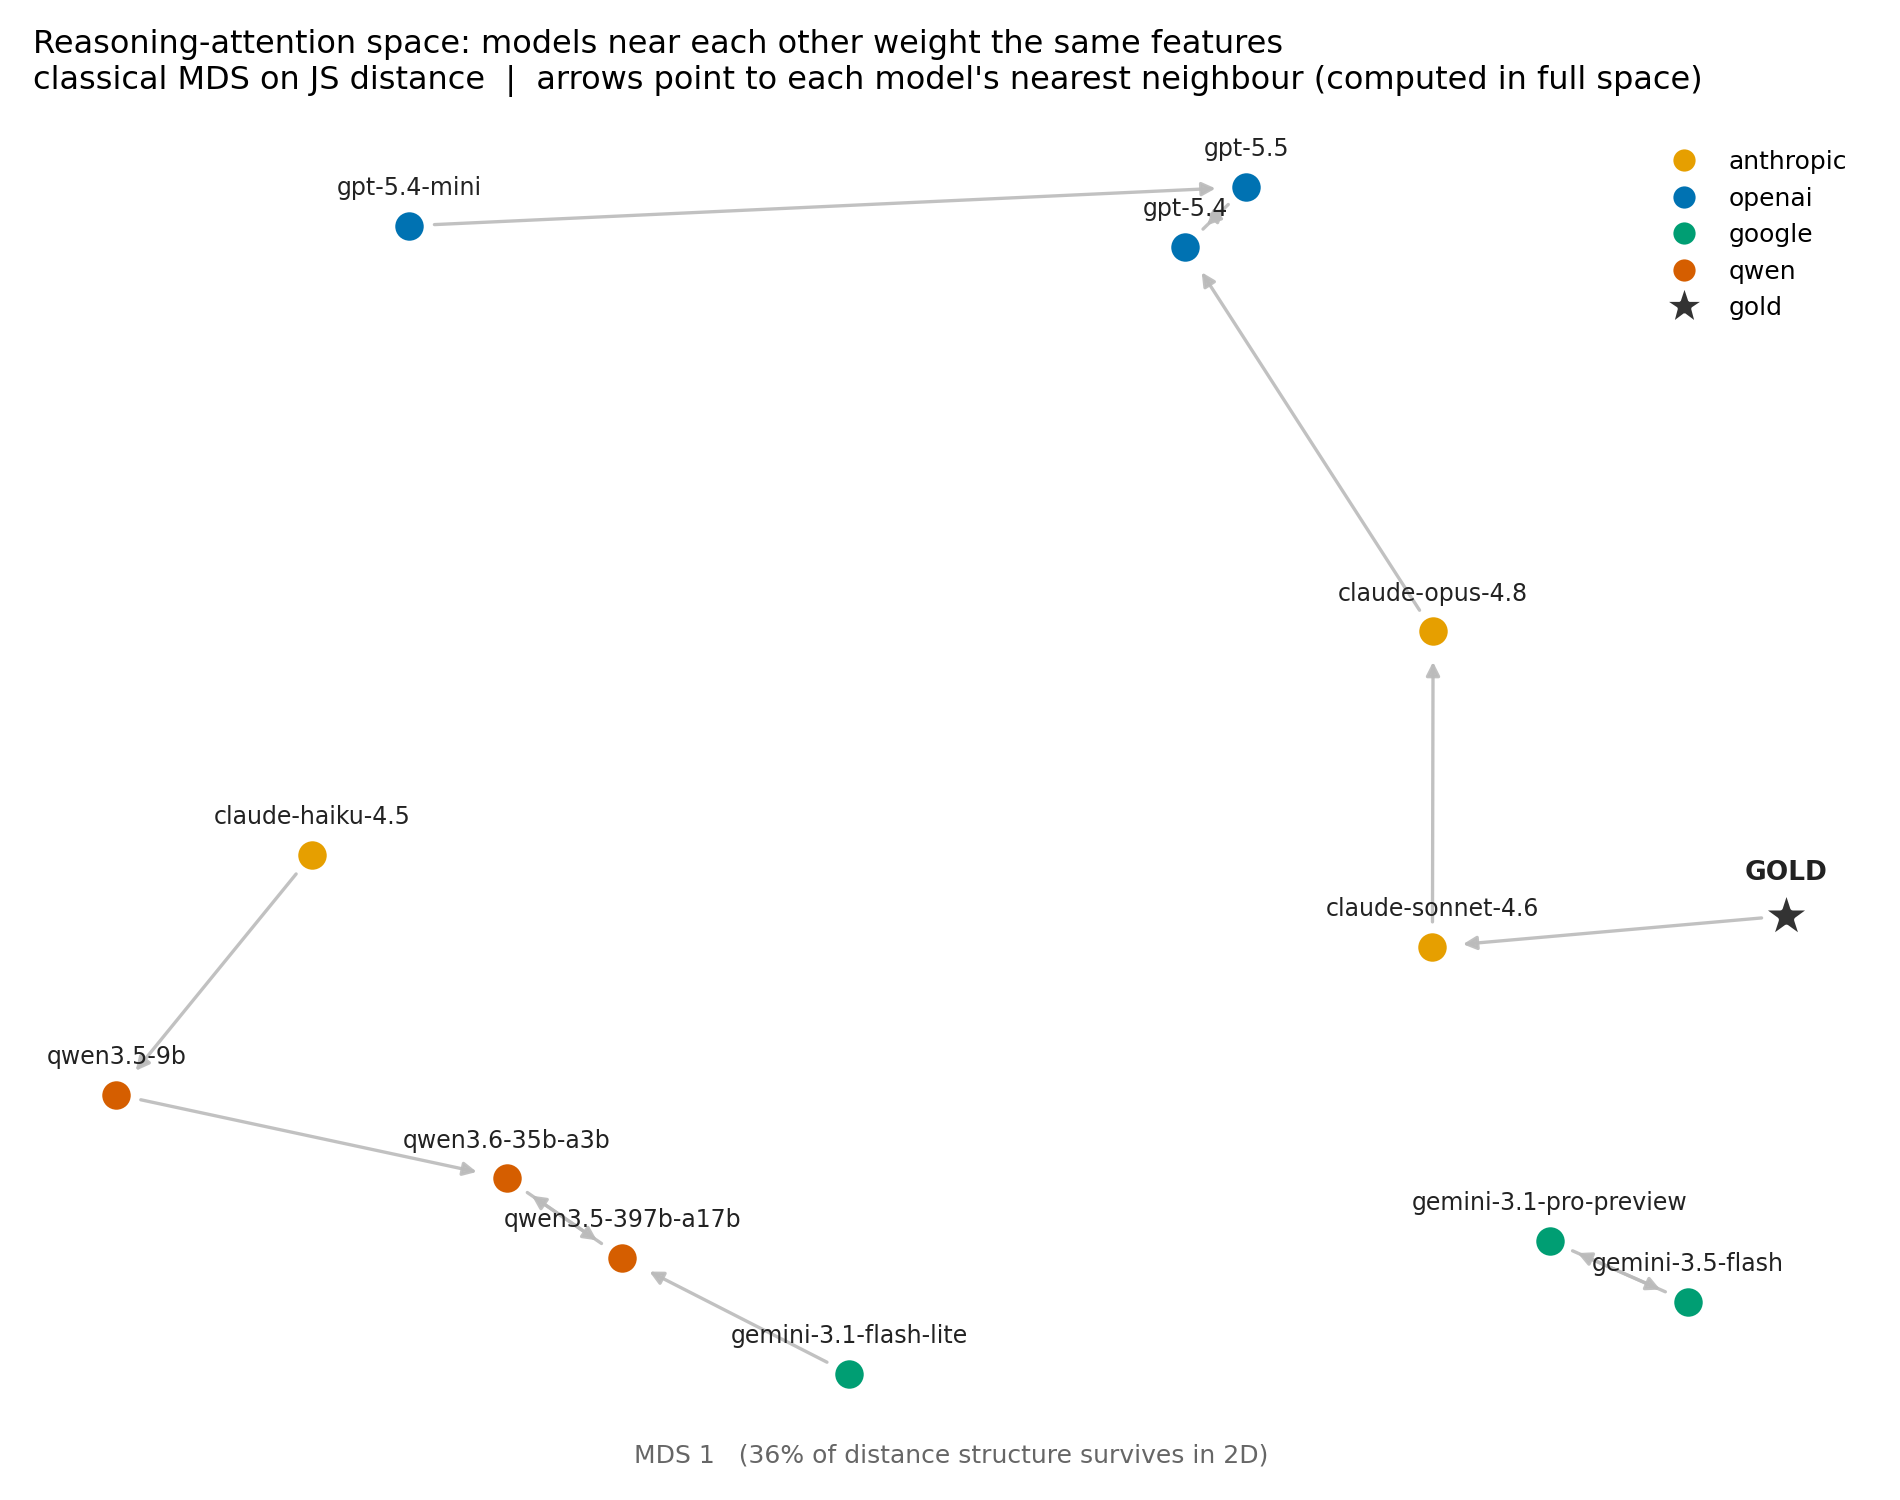
\includegraphics[width=0.82\linewidth]{nn_embedding_freq.png}
\caption{Reasoning-attention space (classical MDS on JS distance of selection-frequency
profiles). Same-family models fall near one another; \texttt{gold} (star) sits inside the
Anthropic neighbourhood. Arrows point to each model's nearest neighbour (computed in the full
space).}
\label{fig:embed}
\end{figure}

\begin{figure}[t]
\centering
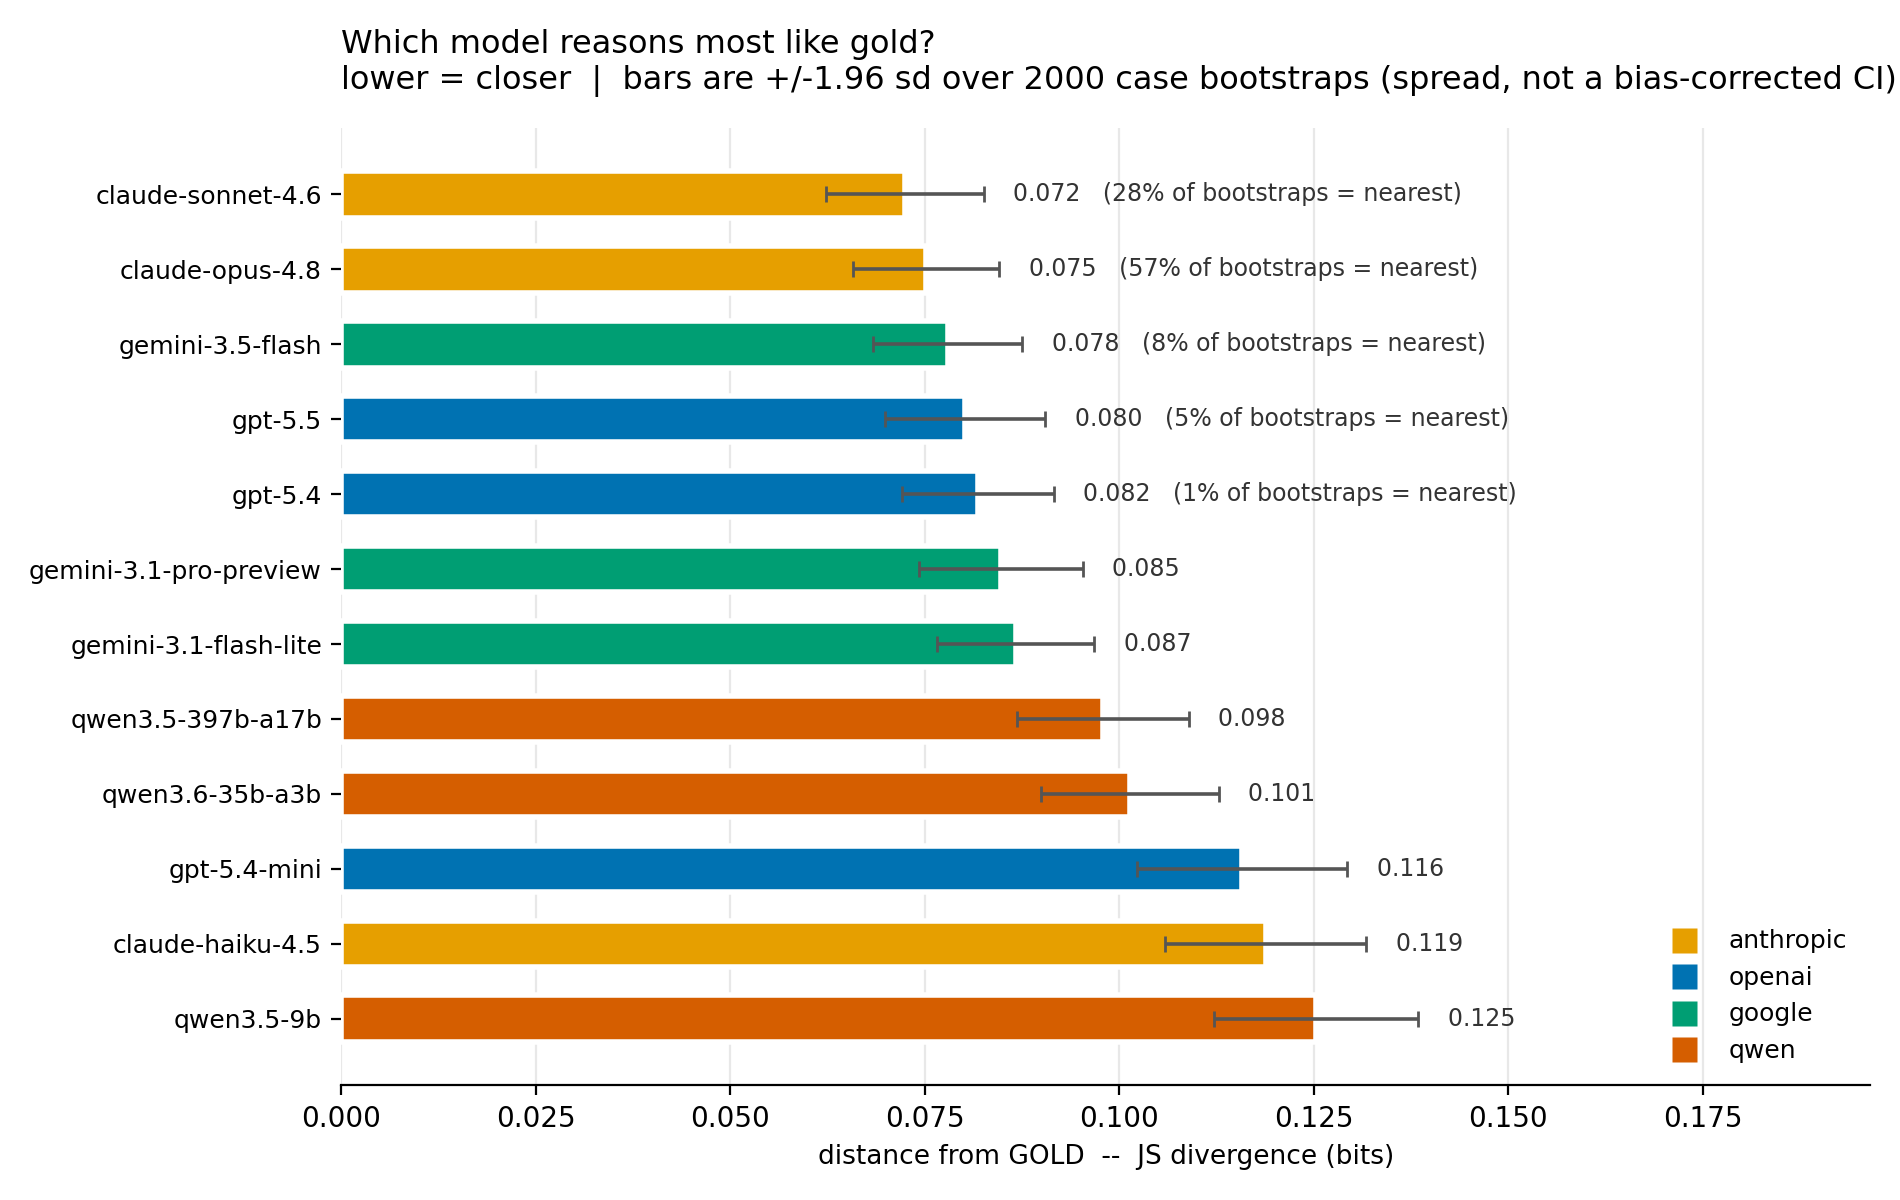
\includegraphics[width=0.82\linewidth]{gold_ranking_freq.png}
\caption{Distance from \texttt{gold} to each model (JS divergence; lower $=$ closer). Anthropic
sonnet-4.6 and opus-4.8 reason most like the reference; small open-weight models are farthest.
Bars are $\pm 1.96$ sd over case bootstraps.}
\label{fig:goldrank}
\end{figure}

\section{Part 3 -- Reasoning Distribution over a Fixed Codebook}

\textbf{Method.} To rule out that Part~2's clustering is a vocabulary artifact---families
phrasing the same concept differently, split into separate global factors---we re-score every
answer against a fixed \textbf{20-criterion legal codebook} (Appendix~\ref{app:codebook})
curated to be roughly mutually exclusive (e.g.\ \emph{risk alignment}, \emph{concentration},
\emph{conflicts of interest}, \emph{standard of care}, \emph{quantitative suitability},
\emph{senior vulnerability}). One labeler marks each criterion \emph{present} if the reasoning
is substantively engaged---argued through the facts, not merely named. Each model becomes a
20-dimensional presence-rate distribution; the same JSD machinery applies.

\textbf{Family tilts.} Relative to the four-family mean, families over- and under-emphasize
different criteria by a few points of engagement each; ordering criteria by cross-family spread
yields an interpretable ``tilt'' signature per family (Figure~\ref{fig:tilts}), consistent
across a family's three tiers more often than not.

\textbf{Clustering is substance, not vocabulary.} On the clean 20-axis codebook the
across/within-family divergence ratio is $\mathbf{1.69}$ (permutation $p=0.011$). Comparing
granularities from noisy to clean---556 open-vocabulary factors (ratio $1.25$, $p<0.001$)
versus the fixed 20-criterion codebook ($1.69$, $p=0.011$)---the ratio \emph{grows} as the axes
are cleaned (Figure~\ref{fig:ratio}). If family clustering were a phrasing artifact, the fixed
codebook would wash it out; instead it sharpens, indicating the noise was \emph{masking} a
substantive family signal.

\begin{figure}[t]
\centering

\includegraphics[width=\linewidth]{family_tilts.png}
\caption{Per-family engagement tilt: each bar is a family's deviation from the four-family mean
presence rate on a criterion (percentage points), ordered by cross-family spread. Families
systematically over- and under-weight different legal factors.}
\label{fig:tilts}
\end{figure}

\begin{figure}[t]
\centering
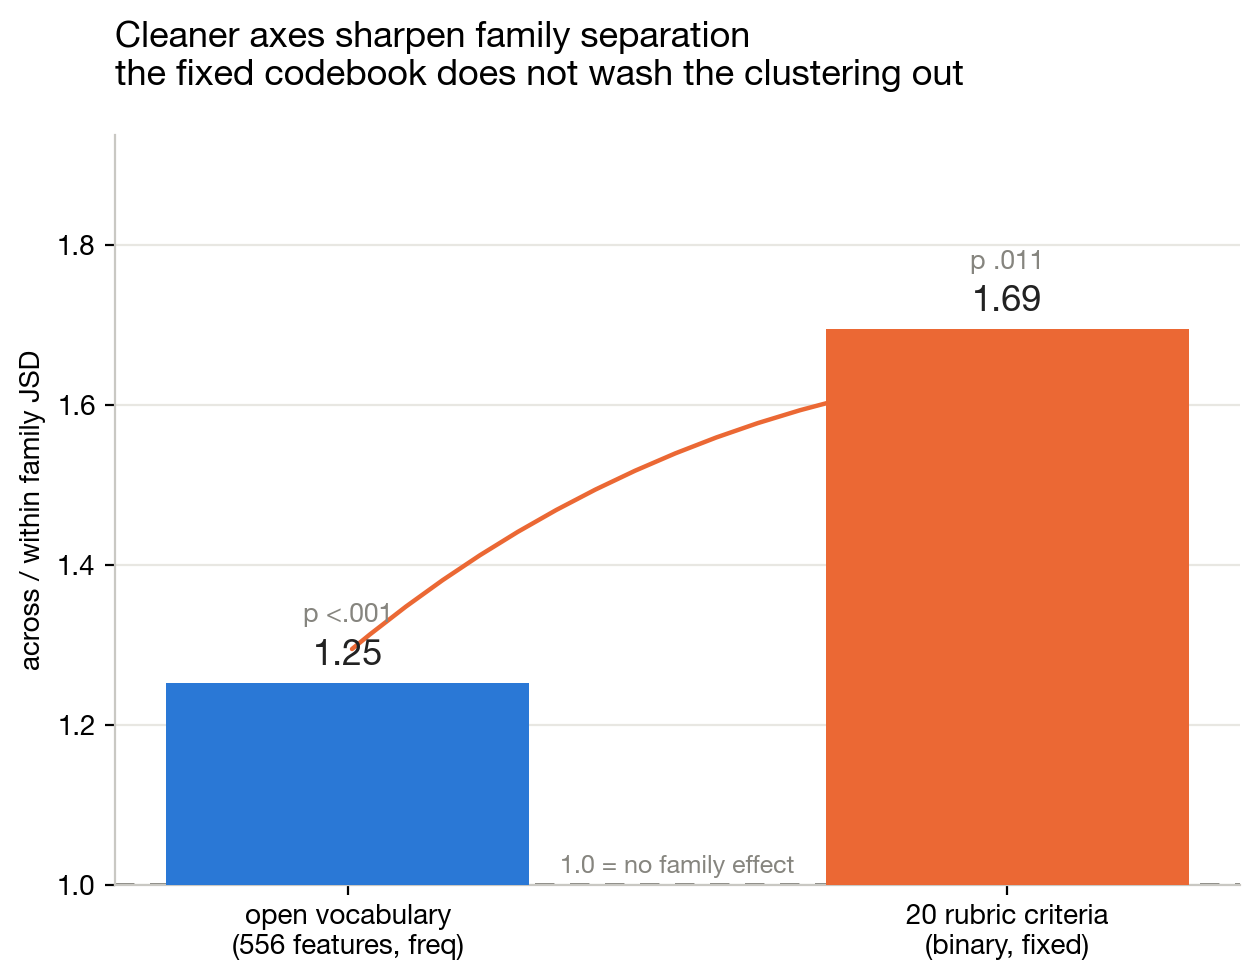
\includegraphics[width=0.62\linewidth]{separation_ratio.png}
\caption{Across/within-family JS-divergence ratio at two granularities. It rises from the open
556-factor vocabulary ($1.25$) to the fixed 20-criterion codebook ($1.69$): cleaning the axes
\emph{sharpens} family separation, so the clustering is substantive, not vocabulary.}
\label{fig:ratio}
\end{figure}

\section{Discussion}

Three patterns cut across the axes. \textbf{First, correctness saturates}: on
clean-ground-truth cases every model reaches the right verdict, so a verdict-only benchmark
would call these models equivalent. \textbf{Second, capability tier lives in the reasoning, not
the verdict}: frontier models cover more factors and match the reference's reasoning more
closely, while small models reach the same verdict on a thinner rationale---precisely the
failure mode a compliance reviewer cares about. \textbf{Third, developer family is a
first-class axis of variation}: models from the same lab reason alike---engaging and weighting
legal factors similarly---more than models of the same size across labs, and this holds on a
fixed, human-curated codebook. Practically, this cautions against treating ``an LLM'' as
interchangeable in a compliance workflow: model choice imports a house reasoning style,
including which factors tend to be under-weighted and how freely authorities are cited.

\section{Limitations}

Results are a \textbf{400-case pilot} from single-run generations. Extraction and rubric scoring
use a \textbf{single} labeler (Llama-3.3-70B); the calibrated dimensions (content similarity,
factor recall, extraction) shift with the labeler even where the outcome metric does not, so
family-level claims should be replicated across labelers (the pipeline supports multiple
extractors/judges). Absolute JSD is biased at this sample size---hence the reliance on rankings
and permutation nulls. The canonicalization arbiter is itself an Anthropic model, a possible
source of mild Anthropic-favouring vocabulary bias, which Part~3's model-free codebook is
designed to neutralize. Finally, roughly $0.1$--$2.5\%$ of extractor / judge calls fail on
malformed JSON and are dropped; the losses are labeler-side and approximately random across
models.

\section{Conclusion}

Verdict correctness is a weak lens on LLM legal-compliance reasoning: it saturates and hides the
differences that matter. Measuring \emph{reasoning coverage} and \emph{reasoning composition} on
a shared benchmark reveals that capability tier and---strikingly---developer family are legible
in how models reason, not just what they conclude. We release the three-axis pipeline to support
reasoning-level evaluation in regulated domains.

% ---------------------------------------------------------------------
% References. Illustrative -- verify and complete before submission.
% (Uses a manual bibliography so the file compiles without a .bib.)
% ---------------------------------------------------------------------
\begin{thebibliography}{9}
\bibitem[Zheng et al.(2023)]{zheng2023judging}
L.~Zheng et al.
\newblock Judging {LLM}-as-a-{J}udge with {MT}-{B}ench and {C}hatbot {A}rena.
\newblock In \emph{NeurIPS}, 2023.

\bibitem[Lin(1991)]{lin1991divergence}
J.~Lin.
\newblock Divergence measures based on the {S}hannon entropy.
\newblock \emph{IEEE Transactions on Information Theory}, 37(1):145--151, 1991.

\bibitem[FINRA / SEC]{finra2111}
FINRA Rule 2111 (Suitability); U.S. SEC Regulation Best Interest (Reg BI),
17~CFR~\S240.15l-1.

\bibitem[Placeholder(a)]{placeholder_faithfulness}
\emph{(placeholder)} Survey on reasoning-faithfulness evaluation of LLMs.

\bibitem[Placeholder(b)]{placeholder_similarity}
\emph{(placeholder)} Behavioural / representational model-similarity methods.
\end{thebibliography}

\appendix

\section{The 20-criterion codebook (abbreviated)}
\label{app:codebook}
\begin{enumerate}\itemsep0pt
\item Risk alignment of product with client profile
\item Concentration / position size \& diversification
\item Time horizon, age \& duration fit
\item Conflicts of interest \& disclosure adequacy
\item Client objectives, risk tolerance \& KYC adequacy
\item Affordability / capacity to bear loss
\item Adequacy of information conveyed
\item Applicable standard of care
\item Fees, costs \& cost--benefit reasonableness
\item Client understanding \& informed consent
\item Affirmative misstatement / misleading conduct
\item Investment experience \& sophistication
\item Consideration of reasonable alternatives
\item Liquidity needs \& emergency reserves
\item Client direction / unsolicited trades
\item Quantitative suitability / excessive trading
\item Reasonable basis \& due diligence
\item Product characteristics, mechanics \& complexity
\item Firm supervision \& recordkeeping integrity
\item Senior status, vulnerability \& diminished capacity
\end{enumerate}

\section{Additional figures}
\label{app:figures}
Figure~\ref{fig:heatmap} shows the raw pairwise divergence matrix behind
Figures~\ref{fig:embed}--\ref{fig:goldrank}; Figure~\ref{fig:modeltilts} gives the per-model
tilt (the three tiers within each family); Figure~\ref{fig:bars} shows the absolute
within/across-family divergence in both feature spaces.

\begin{figure}[h]
\centering
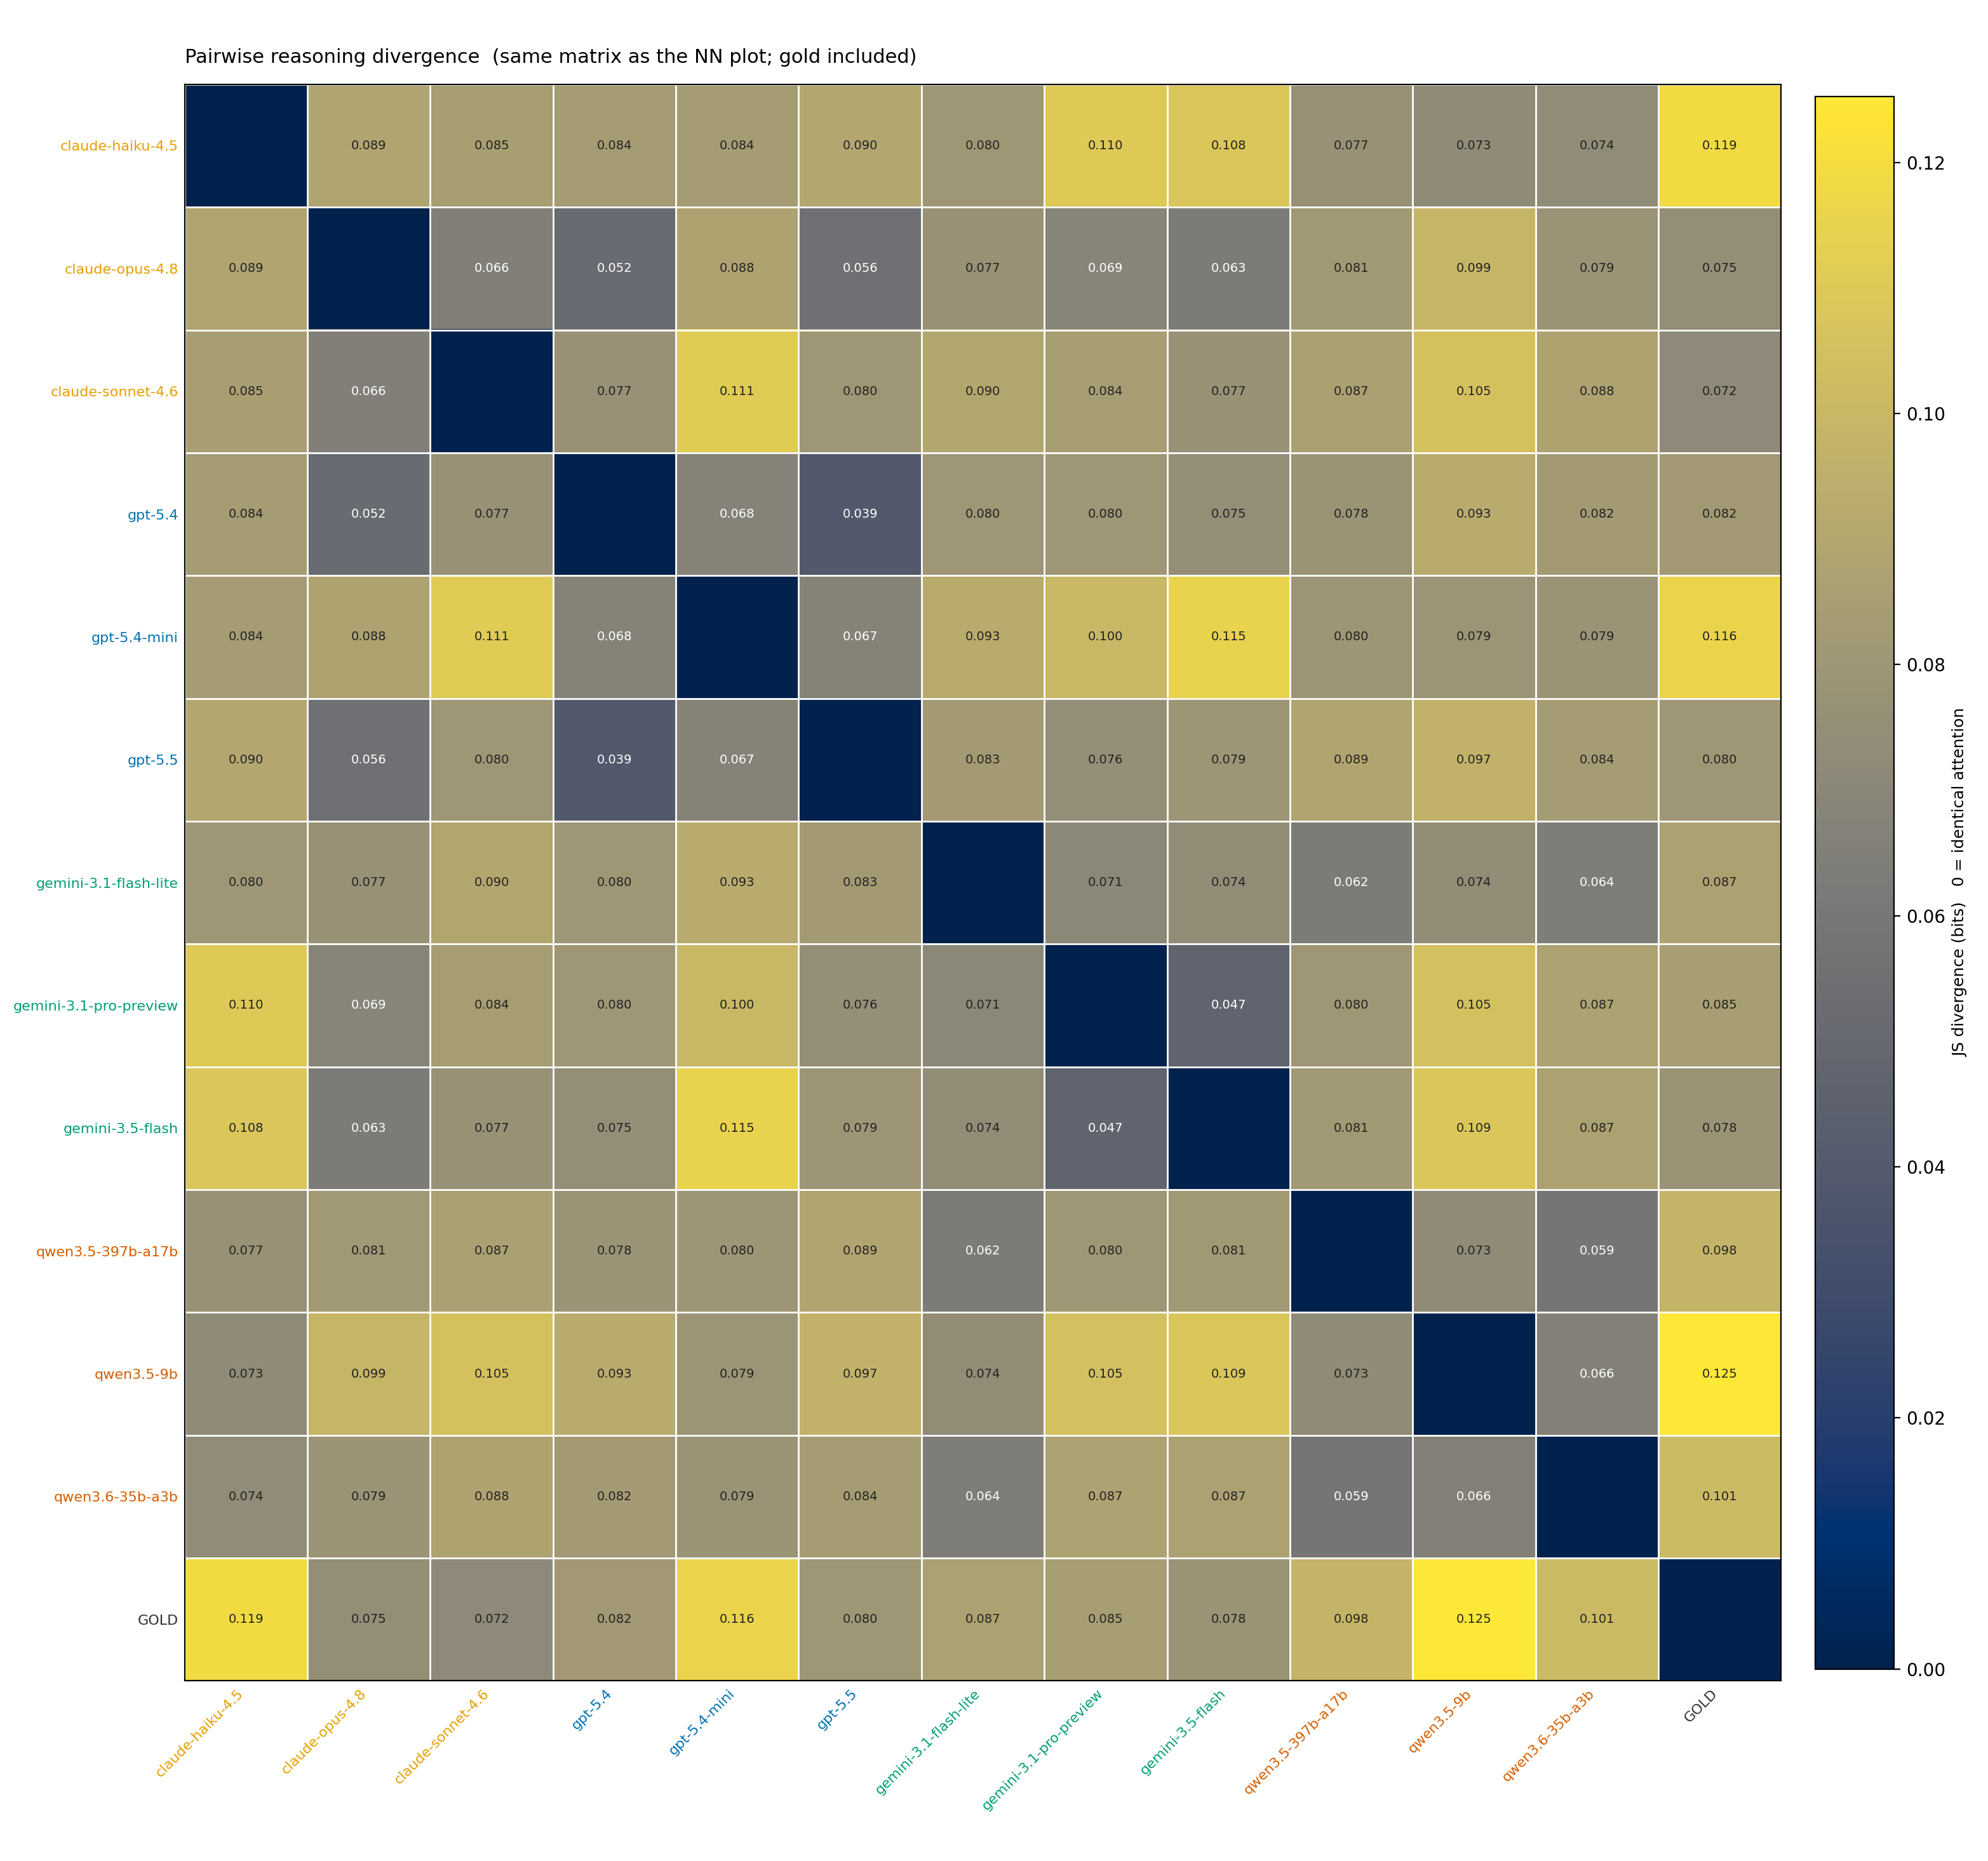
\includegraphics[width=0.72\linewidth]{js_heatmap_freq.png}
\caption{Pairwise JS-divergence heatmap (family-ordered, \texttt{gold} included). Same-family
blocks are consistently lower.}
\label{fig:heatmap}
\end{figure}

\begin{figure}[h]
\centering

\includegraphics[width=\linewidth]{model_tilts.png}
\caption{Per-model engagement tilt, grouped by family. A family's three tiers tend to tilt
together, evidence of a coherent family signature.}
\label{fig:modeltilts}
\end{figure}

\begin{figure}[h]
\centering

\includegraphics[width=0.85\linewidth]{within_across_bars.png}
\caption{Within- vs.\ across-family mean pairwise JSD, in the open-vocabulary (556-factor) and
20-criterion spaces. Across-family pairs diverge more in both.}
\label{fig:bars}
\end{figure}

\end{document}
